%% ============================================
%% ================ Preambule =================
%% ============================================
\documentclass[]{scrartcl}
\usepackage[margin = 0.5in]{geometry}

\usepackage[pdftex,unicode, 
colorlinks=true,
linkcolor = blue]{hyperref}	% нумерование страниц, ссылки!!!!ИМЕННО В ТАКОМ ПОРЯДКЕ СО СЛЕДУЮЩИМ ПАКЕТОМ
%\usepackage[warn]{mathtext}				% Поддержка русского текста в формулах
\usepackage[T1, T2A]{fontenc}			% Пакет выбора кодировки и шрифтов
\usepackage[utf8]{inputenc} 			% любая желаемая кодировка
\usepackage[english, russian]{babel}		% поддержка русского языка
\usepackage{wrapfig}					% Плавающие картинки
\usepackage{amssymb, amsmath}			% стилевой пакет для формул
\usepackage{algorithm}
\usepackage{algorithmic} 
\usepackage{mathtools}


\ifpdf
\usepackage{cmap} 				% чтобы работал поиск по PDF
\usepackage[pdftex]{graphicx}
%\usepackage{pgfplotstable}		% Для вставки таблиц.
\pdfcompresslevel=9 			% сжимать PDF
\else
\usepackage{graphicx}
\fi


\newcommand{\tit}[1]{%
\textit{#1}%
}

\newcommand{\br}[1]{%
\left( #1 \right)%
}

\newcommand{\abs}[1]{%
\left| #1 \right| %
}

\DeclareMathOperator{\tr}{tr}

\mathtoolsset{showonlyrefs=true}

\graphicspath{{./figures/}}
\usepackage{subcaption}
%% ============================================
%% ================ Info =================
%% ============================================
\title{Neural ODE studying}
\author{\begin{tabular}{c c}
	  	 Ilya Lopatin & Daniil Merkulov \\
		 \texttt{lopatin.ia@phystech.edu } & \texttt{daniil.merkulov@skoltech.ru} 
		\end{tabular}}
\date{Project Proposal}

\begin{document}

\maketitle

\begin{abstract}
Проект посвящен изучению принципов работы нейросетевой архитектуры Neural ODE, представленной в работе \cite{NeuralODE}. Планируется проведение различных численных экспериментов с данной архитектурой и последующие объяснение и интерпретация полученных результатов, изучение возможных приложений Neural ODE, таких как: восстановление функции динамики по зашумленным наблюдениям, непрерывные нормализующие потоки, генеративные функции для моделирования временных рядов.
\end{abstract}

\section{Описание}
\subsection{Идея нейросети как обыкновенного дифференциального уравнения}
В этом разделе изложена основная идея построения архитектуры Neural ODE, которая впервые была представлена в работе \cite{NeuralODE}.
 
Опишем как архитектура \tit{Residual neural network} может быть связана или интерпретирована в терминах обыкновенных дифференциальных уравнений (более подробно см. \cite{NeuralODE, OptNet_diff_opt, arbitr_deep_ResNN} ). Рассмотрим общий вид \eqref{eq:skip-connection} \tit{skip-connection} слоя в остаточной нейронной сети:
\begin{equation} \label{eq:skip-connection}
z(t+1) = z(t) + f_t (z (t), \theta ),
\end{equation}
где $t \in \mathbb{N}_0$ -- дискретный параметр, соответствующий номеру слоя, $f_t$ -- передаточная функция узла с номером $t$ ($f: \mathbb{R}^d \to \mathbb{R}^d$, где $d$ -- размерность $z$ ), $\theta$ -- множество, <<обучаемых>> параметров нейронной сети.Наряду с этим, рассмотрим задачу Коши \eqref{eq:Koshi_standart_task} для обыкновенного дифференциального уравнения:
\begin{equation} \label{eq:Koshi_standart_task}
\left\{ \begin{aligned}
			& \frac{d z(t) }{dt} = f(z(t), t, \theta) \\
			& t \in [t_1 ; t_2] \\
			& z(t_1) = x
		\end{aligned} \right.
\end{equation}
и явный метод Эйлера \eqref{eq:Euler_standart_method} численного решения \eqref{eq:Koshi_standart_task}:
\begin{equation} \label{eq:Euler_standart_method}
z(t+\Delta t) = z(t) + \Delta t f(z(t), t, \theta), ~ z(t_1) = x,
\end{equation}
где $\Delta t$ -- параметр численной схемы, соответствующий длине шага сетки численного решения. Заметим, что при $\Delta t = 1$ \eqref{eq:skip-connection} и \eqref{eq:Euler_standart_method} полностью совпадают.
Основная идея состоит в том, чтобы интерпретировать нейронную сеть как задачу Коши \eqref{eq:Koshi_standart_task}. Оказывается, что при таком подходе процедуры прямого и обратного распространения можно представить в виде численного решения задачи Коши для ОДУ.
 
\subsection{Прямое и обратное распространение}
Прямое распространение представляет численное решение \eqref{eq:Koshi_standart_task}, отметим, что решение необязательно проводить именно методом Эйлера, здесь применимы методы более высокого порядка и устойчивости, например методы Рунге-Кутты (для справки по численным методам  см., например, \cite{RK_method}). Вообще, здесь можно отметить, что, если рассматривать т.н. \tit{dense neural network}, сигнал в которых на $k$-том слое явно зависит не только от сигнала на $k-1$--слое, но и предыдущих, иначе говоря в формулу \eqref{eq:skip-connection} явно входят   $z(t-1), z(t-2), \dots , z(t-k) $, то аналогия между прохождением сигнала в таких нейросетях и маршевыми методами Рунге-Кутты становится еще сильнее. 

Для алгоритма обратного распространения в работе \cite{NeuralODE} вводится следующая функция (\tit{adjoint function}\footnote{вообще говоря, понятие сопряженного решения для ОДУ известно достаточно давно и было введено Л.С. Понтрягиным, cм. \cite{PontryaginPrinciples}}):
$$
a(t) = \frac{\partial L(y)}{ \partial z(t) },
$$
где $L(y)$ -- функция потерь (\tit{loss--function}), а $y$ -- выход нейросети (в нашем случае $y=z(t_2)$).

В \cite{NeuralODE} показано, что $a(t)$ есть решение следующей задачи Коши \eqref{eq:adjoiunt_Koshi} (заметим, что условие задано на правом крае, а не на левом, как обычно):
\begin{equation} \label{eq:adjoiunt_Koshi}
\left\{ \begin{aligned}
  		& \frac{d a(t)}{dt} = - a^T(t) \frac{\partial f}{ z(t)} \\
		& a(t_2) = \frac{\partial L}{ \partial y}
\end{aligned} \right.
\end{equation}
А градиент по обучаемым параметрам выражается как:
\begin{equation} \label{eq:grad_loss_theta}
 \nabla_{\theta} L = \int_{t_1}^{t_2} a^T(t) \frac{\partial f}{\partial \theta} \left( z(t), t, \theta \right) dt,
\end{equation}
где подынтегральное выражение представляет  
Ниже представлен алгоритм из \cite{NeuralODE}, подсчета всех необходимых градиентов. 

\begin{figure}[h!]
\centering
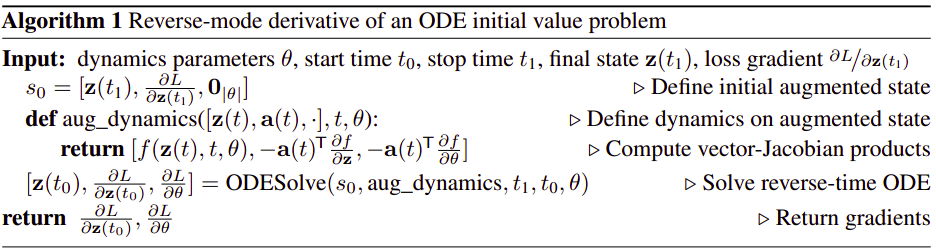
\includegraphics[width= 0.95 \linewidth]{grad_alg.png}
\end{figure}

где $f_{aug}$ -- расширенная или \textit{аугментированная} функция динамики:
$$
\frac{d}{dt} \begin{bmatrix}
z \\
\theta \\
t
\end{bmatrix} (t) = f_{aug} \left( \left[ z, \theta, t \right]  \right) = \begin{bmatrix}
f \left(  \left[ z, \theta, t \right] \right) \\
0 \\
1
\end{bmatrix}
$$

\subsection{Нормализующие потоки}
В работе \cite{modecollapse} показано, что для генеративно-состязательных нейросетей (\textit{GAN}) фактически неизбежен т.н. \tit{Mode Collapse} -- особенность обучения GAN-ов -- нейросеть обучается генерировать изображение или иной выход на основе только лишь части своей обучающей выборки. Один из возможных способов избежать Mode Collapse это подсчитывать плотность распределения, порожденного генератором GAN и регуляризация каким-либо способом, если плотность становится сильно неравномерной, подробное изложение см. в \cite{normalizing_flows}. Однако этот способ имеет следующую вычислительную трудность: рассмотрим моделирование плотности сложного распределения в высокоразмерном пространстве как прохождение распределения $z(0) \sim p_0 (z_0)$ через нелинейное преобразование -- нейросеть с $T$ слоями: $z(T) \sim  p_T (z (T) )$, тогда есть возможность посчитать плотность трансформированного распределения по формуле \eqref{eq:calcul_prob_density} 
\begin{equation} \label{eq:calcul_prob_density}
\log p_T \br{ z(T) } = \log p_0 \br{ z(0) }  - \sum_{t=1}^T \abs{ \frac{ d f_t }{ d f_{t-1} } },
\end{equation}    
где $z(T) = f( z(0), \theta )$ -- прямое распространение в нейронной сети, а $ \abs{ d f_t / d f_{t-1}  } $ -- якобиан между соответствующими слоями, вычисление которого есть куб операций от размерности пространства $\Theta (d^3)$, что делает формулу \eqref{eq:calcul_prob_density} неприменимой на практике в общем случае для высокоразмерных пространств.

Здесь оказывается полезным следующие утверждение:

\tit{Пусть $z(t)$ -- конечная непрерывная случайная величина
с вероятностью  $p(z(t))$, зависящей от времени. Пусть $dz / dt = f(z(t), t)$ -- дифференциальное уравнение, описывающее непрерывное во времени преобразование $z(t)$. Предполагая, что $f$ удовлетворяет условию Липшица по аргументу  $z$ и непрерывна по аргументу $t$, имеем следующее соотношение} \eqref{eq:ODE_prob_trace}:
\begin{equation} \label{eq:ODE_prob_trace}
 \frac{\partial \log p \br{z(t)} }{\partial t } = - \tr \br{ \frac{\partial f }{ \partial z(t) }   }
 \end{equation} 
\subsection{Преимущества и приложения}
Отметим несколько преимуществ данной архитектуры. Варьируя шаг численного решения ОДУ, мы как бы меняем число слоев в нейросети, т.е. архитектура Neureal ODE дает возможность фактически в режиме реального времени производить трейд-ин между точностью и временем работы. Кроме того, заметим, что ввиду метода подсчета градиента нету необходимости хранить все результаты прохождения в скрытых слоях, т.е. процедура градиентного спуска в данной архитектуре константна по памяти относительно количества слоев или мелкости сетки численного решения. Более подробно: численно решается \eqref{eq:adjoiunt_Koshi}, если решение происходит методом Рунге-Кутты, то необходимо помнить только фиксированное число предыдущих значений, полученные численные значения можно сразу передавать в \eqref{eq:grad_loss_theta} для подсчета $\nabla_{\theta} L$.

Поговорим о возможных приложениях:
\begin{itemize}
\item Замена Res-блока на блок NeuralODE с целью указанных выше преимуществах.
\item Восстановление функции динамики. Пусть у нас есть какая-то динамическая система с законом типа $z'(t) = f(z(t), t)$, где $f$ -- неизвестная функция динамики и есть серия наблюдений точек траектории. Тогда можно попытаться восстановить эту функцию динамики, надлежащем образом обучив NeuralODE.
\item Непрерывные Нормализующие Потоки. Семплирование плотности распределения какого-то сложного процесса может помочь например в регуляризации обучения нейронных сетей архитектуры GAN.
\end{itemize} 

\section{Problem}
Итак, мы имеем достаточно новую архитектуру (работа \cite{NeuralODE} вышла 2018 году) нейронной сети. Целью этого проекта является экспериментальное изучение следующих вопросов: 
\begin{itemize}
\item Действительно ли NeuralODE имеет все указанные выше преимущества?
\item Как NeuralODE ведет себя в плане точности распознавания / времени обучения, требуемой памяти по сравнению со стандартными остаточными нейросетями?
\item Как точно NeuralODE может восстановить неизвестные динамики по серии наблюдений и сколько временных ресурсов и памяти на это нужно?
\item Как точно NeuralODE может семплировать плотность распределения сложных процессов? Какие могут быть ограничения на целевую плотность?  
\end{itemize}
Отметим, что, теоретически можно указать <<слабые места>> данной архитектуры. Что если скрытая целевая функция динамики плохо обусловленна возможно ли в таких случаях корректно обучить нейросеть? При выводе формулы \eqref{eq:ODE_prob_trace} берется бесконечно малое приращение аргументов, мы же, хоть и можем варьировать шаг решения, не можем делать его <<слишком малым>> ввиду, например, ресурсных ограничений, применима ли формула \eqref{eq:ODE_prob_trace} для реальных вычислений, получим ли мы действительно выигрыш или лучше вернуться к подходу, основанному на формуле \eqref{eq:calcul_prob_density}?

\section{Outcomes}
В качестве выхода планируется репозиторий на github с авторской реализацией NeuralODE из статьи \cite{NeuralODE}, плюс результаты экспериментов, проведенных с этой архитектурой. Быть может, будет сделан отчет в формате статьи / доклада с описанием и интерпретированием полученных  результатов.

Эксперименты планируется проводить для ответов  на поставленные вопросы в разделе <<Problem>>. Ниже ориентировочный список основных сценариев:
\begin{itemize}
\item Запуск и сравнение результатов (точность / время / память) с другими известными нейросетями. Например, задача классификации с обучающей выборкой MNIST.
\item Задание несколько различных функций динамик и отслеживание, как Neural ODE будет обучаться/восстанавливать их по множеству точек.
\item Проверка (желательно даже визуализация процесса), как Neural ODE будет моделировать заранее заданную плотность распределения.
\end{itemize} 

\section{Литературный обзор}
Работа \cite{NeuralODE} есть основная в моем проекте, в ней была впервые построена архитектура NeuralODE. Работы \cite{OptNet_diff_opt}, \cite{arbitr_deep_ResNN} являются фундаментом для работы \cite{NeuralODE}, в них были описаны первые аналогии между ResNet и дифференциальными уравнениями.Хочется отметить \cite{PontryaginPrinciples} в этой работе группа советских математиков во главе с Л.С. Понтрягиным впервые ввела технику сопряженных функций, вывод формулы \eqref{eq:grad_loss_theta} идейно вдохновлен этой работой. Работа \cite{RK_method} содержит описания существующих численных метод решения ОДУ, в частности особо интересные для этой работы методы Рунге-Кутты.  В работе \cite{normalizing_flows} был предложен метод моделирования сложной плотности с помощью нормализующих потоков. В работе \cite{modecollapse} подробно изложена проблема Mode Collapse для генеративно-состязательных нейронных сетей. В работе \cite{CasADi} рассматриваются методы компьютерного подсчета выражений типа \eqref{eq:adjoiunt_Koshi},\eqref{eq:grad_loss_theta} содержащие пространственные якобианы больших размерностей.

\section{Метрики качества}
В качестве метрик качества можно рассмотреть содержания планируемого репозитория: количество, широта и результаты проведенных экспериментов по  применению Neural ODE. Под широтой подразумевается:
\begin{itemize}
\item планируется провести несколько серий экспериментов для проверки различных способов применения Neural ODE (см. раздел <<Преимущества и приложения>>), в идеале планируется проверить все указанные применения с различными типами входных данных.
\item на каждый вопрос, поставленный в разделе Problem, можно будет дать ответ, подкрепленный соответствующими тестами.
\end{itemize}  
Качество проделанной работы можно будет оценить по результат экспериментов, как точно они согласуются с теоретическими предсказаниями и насколько хорошо их можно объяснить. 

\section{Примерный план}
\begin{itemize}
	\item Сначала, конечно, необходимо ознакомиться с теоретическим аспектом работы NeuralODE: прочитать оригинальную статью и, быть может, пару других постов/обзорных статей, благо материала много. Т.к. теоретический материал мне знаком в достаточной степени хорошо я выделю на это сравнительно малый срок: до 22 апреля (т.е. до \tit{draft 1} ). Особое внимание я уделю нормализующим потокам т.к. на данный момент это самая сложная для меня теоретическая тема в данном проекте.
	\item Потом планирую установить и запустить оригинальный репозиторий и разобрать вложенные в него примеры. В этом пункте я подразумеваю просто "технический" запуск кодов, поэтому выделю на это время до 25 апреля.
	\item До 29 апреля (т.е. draft 2) планируется провести первые собственные эксперименты, чтобы понять "что к чему". Планируется начать с экспериментов по восстановлению скрытых функций динамик.
	\item К 6 мая планируется расширить число экспериментов, провести серию экспериментов в сфере нормализующих потоков. Быть может, реализовать некоторую часть репозитория самостоятельно, это может быть например реализация <<с нуля>> какого-то одно приложения, на данный момент, самым простым кажется восстановление функции динамики.
	\item После 6 мая, по согласованию с семинаристом планируется расширение проекта в какую-то из сторон, указанных в пункте выше.  
\end{itemize}

\bibliographystyle{unsrt}
\bibliography{biblio}

\end{document}
